\documentclass[18pt]{article}
\usepackage{tikz}
\usetikzlibrary{positioning}
\usepackage{pdflscape}

\usepackage{geometry}
\geometry{top=5cm,bottom=0cm,left=5cm,right=5cm}
\usetikzlibrary{arrows}

\begin{document}
\pagestyle{empty}

\begin{landscape}
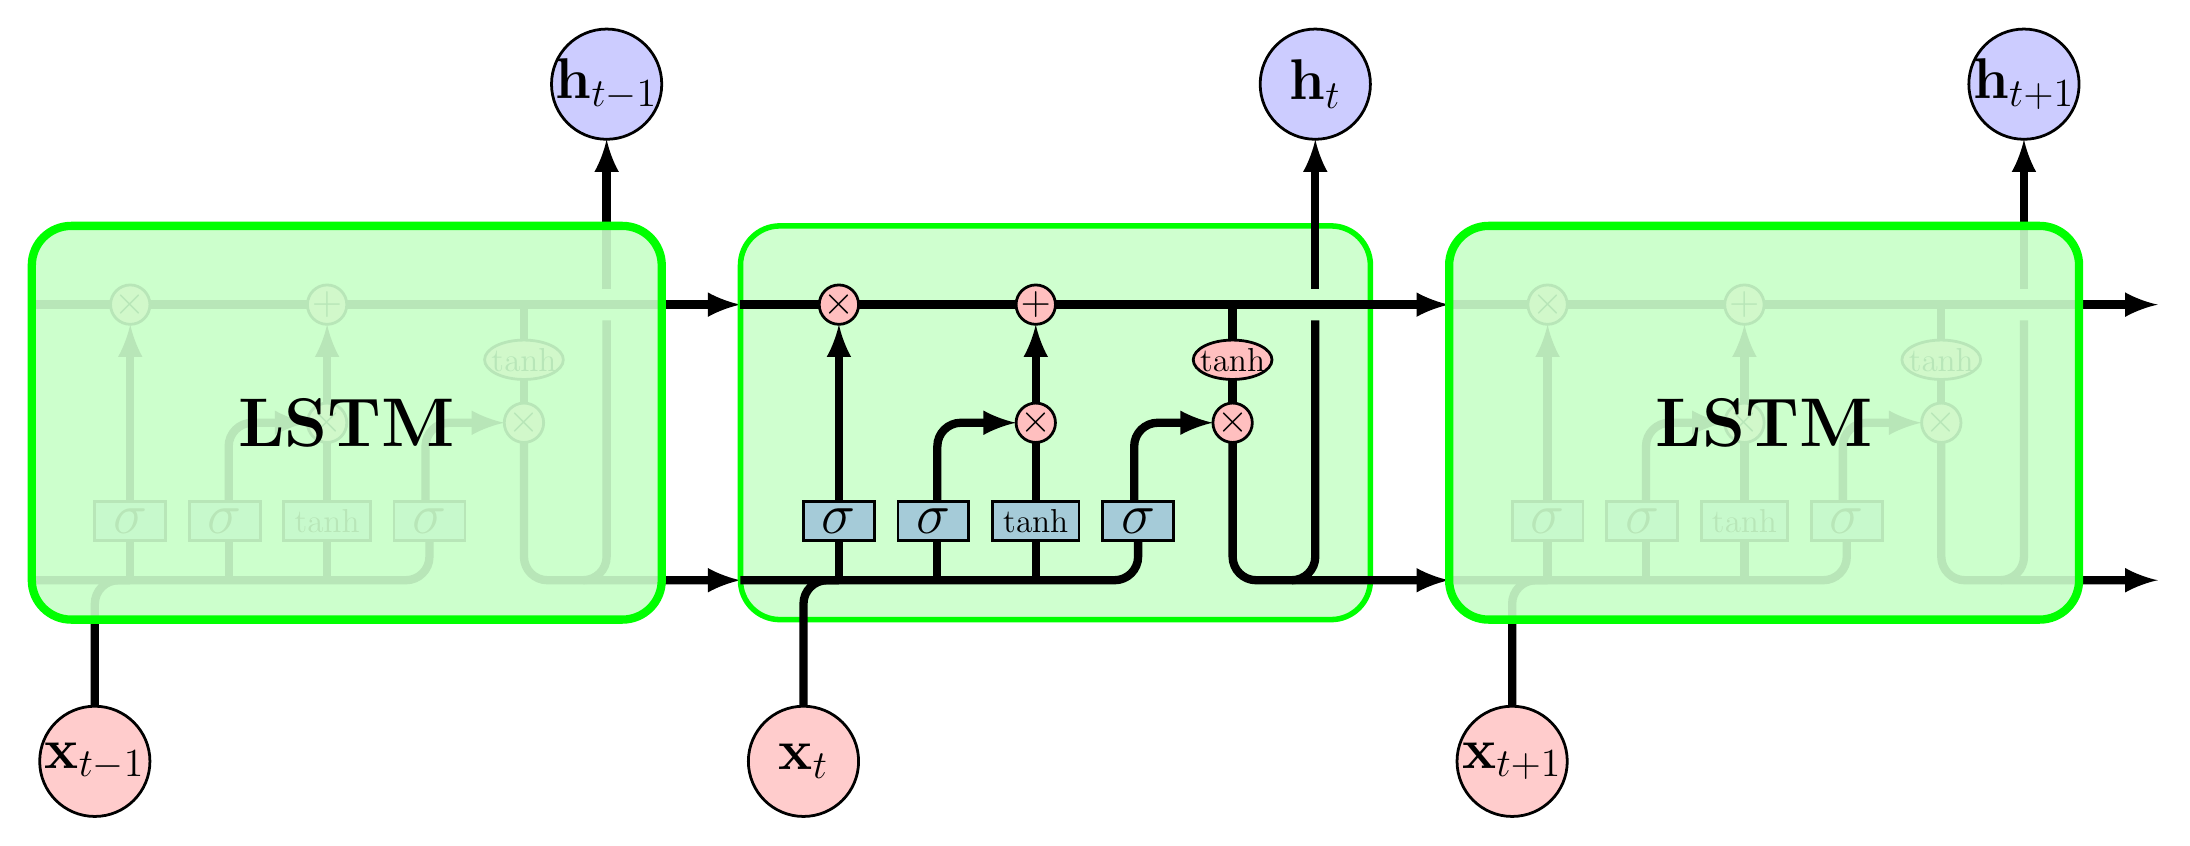
\begin{tikzpicture}
\coordinate (O) at (0, 0);

\def\offset{0}
% input
\filldraw[fill = red,fill opacity=0.2,draw=black,line width=1pt] (-1.2+\offset,0.7) circle (0.7) node[fill opacity=1]{\huge $\mathbf{x}_{t-1}$};

%LSTM
\filldraw[fill={rgb,255:red,204; green,255; blue,204},fill opacity=0.95,draw=green,line width=2pt,rounded corners=0.5cm] (-2+\offset,2.5) rectangle (6+\offset,7.5); % background
\filldraw[fill=blue,fill opacity=0.2,draw=black,line width=1pt] (-1.2+\offset,3.5) rectangle (-0.3+\offset,4)node[pos=.5,fill opacity=1]{\huge $\sigma$};

\filldraw[fill=blue,fill opacity=0.2,draw=black,line width=1pt] (0+\offset,3.5) rectangle (0.9+\offset,4)node[pos=.5,fill opacity=1]{\huge $\sigma$};

\filldraw[fill=blue,fill opacity=0.2,draw=black,line width=1pt] (1.2+\offset,3.5) rectangle (2.3+\offset,4)node[pos=.5,fill opacity=1]{\large tanh};

\filldraw[fill=blue,fill opacity=0.2,draw=black,line width=1pt] (2.6+\offset,3.5) rectangle (3.5+\offset,4)node[pos=.5,fill opacity=1]{\huge $\sigma$};

\filldraw[fill=pink,fill opacity=1,draw=black,line width=1pt] (-0.75+\offset,6.5) circle (0.25)node[fill opacity=1]{\Large $\times$};

\filldraw[fill=pink,fill opacity=1,draw=black,line width=1pt] (1.75+\offset,5) circle (0.25)node[fill opacity=1]{\Large $\times$};

\filldraw[fill=pink,fill opacity=1,draw=black,line width=1pt] (4.25+\offset,5) circle (0.25)node[fill opacity=1]{\Large $\times$};

\filldraw[fill=pink,fill opacity=1,draw=black,line width=1pt] (1.75+\offset,6.5) circle (0.25)node[fill opacity=1]{\Large $+$};

\filldraw[fill=pink,fill opacity=1,draw=black,line width=1pt]  (4.25+\offset,5.8) ellipse (0.5cm and 0.25 cm) node[fill opacity=1]{\large tanh};

\draw[ultra thick,black,rounded corners=0.3cm,line width=3pt] (-1.2+\offset,1.4)-- (-1.2+\offset,3)-- (-0.75+\offset,3);
\draw[ultra thick,black,rounded corners=0.3cm,line width=3pt] (-2+\offset,3)-- (3.05+\offset,3)-- (3.05+\offset,3.5);
\draw[ultra thick,black,line width=3pt] (-0.75+\offset,3)-- (-0.75+\offset,3.5);
\draw[-latex,black,line width=3pt] (-0.75+\offset,4)-- (-0.75+\offset,6.25);

\draw[ultra thick,black,line width=3pt] (0.5+\offset,3)-- (0.5+\offset,3.5);
\draw[-latex,black,rounded corners=0.3cm,line width=3pt] (0.5+\offset,4)-- (0.5+\offset,5)-- (1.5+\offset,5);

\draw[ultra thick,black,line width=3pt] (1.75+\offset,3)-- (1.75+\offset,3.5);
\draw[ultra thick,black,line width=3pt] (1.75+\offset,4)-- (1.75+\offset,4.75);
\draw[-latex,black,rounded corners=0.3cm,line width=3pt] (1.75+\offset,5.25)-- (1.75+\offset,6.25);

\draw[ultra thick,black,line width=3pt] (-2+\offset,6.5)-- (-1+\offset,6.5);
\draw[ultra thick,black,line width=3pt] (-0.5+\offset,6.5)-- (1.5+\offset,6.5);
\draw[-latex,black,line width=3pt] (2+\offset,6.5)-- (7+\offset,6.5);

\draw[-latex,black,rounded corners=0.3cm,line width=3pt] (3+\offset,4)-- (3+\offset,5)-- (4+\offset,5);

\draw[ultra thick,black,line width=3pt] (4.25+\offset,6.5)-- (4.25+\offset,6.05);
\draw[ultra thick,black,line width=3pt] (4.25+\offset,5.55)-- (4.25+\offset,5.25);
\draw[-latex,black,rounded corners=0.3cm,line width=3pt] (4.25+\offset,4.75)-- (4.25+\offset,3)-- (7+\offset,3);
\draw[ultra thick,black,rounded corners=0.3cm,line width=3pt] (5+\offset,3)-- (5.3+\offset,3) -- (5.3+\offset,6.3);
\draw[-latex,black,line width=3pt] (5.3+\offset,6.7)-- (5.3+\offset,8.6);

\filldraw[fill = blue,fill opacity=0.2,draw=black,line width=1pt] (5.3+\offset,9.3) circle (0.7)node[fill opacity=1]{\huge $\mathbf{h}_{t-1}$};

\filldraw[fill={rgb,255:red,204; green,255; blue,204},fill opacity=0.9,draw=green,line width=3pt,rounded corners=0.5cm] (-2+\offset,2.5) rectangle (6+\offset,7.5)node[pos=.5,fill opacity=1]{\Huge \textbf{LSTM}};


\def\offset{9}
% input
\filldraw[fill = red,fill opacity=0.2,draw=black,line width=1pt] (-1.2+\offset,0.7) circle (0.7) node[fill opacity=1]{\huge $\mathbf{x}_{t}$};

%LSTM
\filldraw[fill={rgb,255:red,204; green,255; blue,204},fill opacity=0.95,draw=green,line width=2pt,rounded corners=0.5cm] (-2+\offset,2.5) rectangle (6+\offset,7.5); % background
\filldraw[fill=blue,fill opacity=0.2,draw=black,line width=1pt] (-1.2+\offset,3.5) rectangle (-0.3+\offset,4)node[pos=.5,fill opacity=1]{\huge $\sigma$};

\filldraw[fill=blue,fill opacity=0.2,draw=black,line width=1pt] (0+\offset,3.5) rectangle (0.9+\offset,4)node[pos=.5,fill opacity=1]{\huge $\sigma$};

\filldraw[fill=blue,fill opacity=0.2,draw=black,line width=1pt] (1.2+\offset,3.5) rectangle (2.3+\offset,4)node[pos=.5,fill opacity=1]{\large tanh};

\filldraw[fill=blue,fill opacity=0.2,draw=black,line width=1pt] (2.6+\offset,3.5) rectangle (3.5+\offset,4)node[pos=.5,fill opacity=1]{\huge $\sigma$};

\filldraw[fill=pink,fill opacity=1,draw=black,line width=1pt] (-0.75+\offset,6.5) circle (0.25)node[fill opacity=1]{\Large $\times$};

\filldraw[fill=pink,fill opacity=1,draw=black,line width=1pt] (1.75+\offset,5) circle (0.25)node[fill opacity=1]{\Large $\times$};

\filldraw[fill=pink,fill opacity=1,draw=black,line width=1pt] (4.25+\offset,5) circle (0.25)node[fill opacity=1]{\Large $\times$};

\filldraw[fill=pink,fill opacity=1,draw=black,line width=1pt] (1.75+\offset,6.5) circle (0.25)node[fill opacity=1]{\Large $+$};

\filldraw[fill=pink,fill opacity=1,draw=black,line width=1pt]  (4.25+\offset,5.8) ellipse (0.5cm and 0.25 cm) node[fill opacity=1]{\large tanh};

\draw[ultra thick,black,rounded corners=0.3cm,line width=3pt] (-1.2+\offset,1.4)-- (-1.2+\offset,3)-- (-0.75+\offset,3);
\draw[ultra thick,black,rounded corners=0.3cm,line width=3pt] (-2+\offset,3)-- (3.05+\offset,3)-- (3.05+\offset,3.5);
\draw[ultra thick,black,line width=3pt] (-0.75+\offset,3)-- (-0.75+\offset,3.5);
\draw[-latex,black,line width=3pt] (-0.75+\offset,4)-- (-0.75+\offset,6.25);

\draw[ultra thick,black,line width=3pt] (0.5+\offset,3)-- (0.5+\offset,3.5);
\draw[-latex,black,rounded corners=0.3cm,line width=3pt] (0.5+\offset,4)-- (0.5+\offset,5)-- (1.5+\offset,5);

\draw[ultra thick,black,line width=3pt] (1.75+\offset,3)-- (1.75+\offset,3.5);
\draw[ultra thick,black,line width=3pt] (1.75+\offset,4)-- (1.75+\offset,4.75);
\draw[-latex,black,rounded corners=0.3cm,line width=3pt] (1.75+\offset,5.25)-- (1.75+\offset,6.25);

\draw[ultra thick,black,line width=3pt] (-2+\offset,6.5)-- (-1+\offset,6.5);
\draw[ultra thick,black,line width=3pt] (-0.5+\offset,6.5)-- (1.5+\offset,6.5);
\draw[-latex,black,line width=3pt] (2+\offset,6.5)-- (7+\offset,6.5);

\draw[-latex,black,rounded corners=0.3cm,line width=3pt] (3+\offset,4)-- (3+\offset,5)-- (4+\offset,5);

\draw[ultra thick,black,line width=3pt] (4.25+\offset,6.5)-- (4.25+\offset,6.05);
\draw[ultra thick,black,line width=3pt] (4.25+\offset,5.55)-- (4.25+\offset,5.25);
\draw[-latex,black,rounded corners=0.3cm,line width=3pt] (4.25+\offset,4.75)-- (4.25+\offset,3)-- (7+\offset,3);
\draw[ultra thick,black,rounded corners=0.3cm,line width=3pt] (5+\offset,3)-- (5.3+\offset,3) -- (5.3+\offset,6.3);
\draw[-latex,black,line width=3pt] (5.3+\offset,6.7)-- (5.3+\offset,8.6);

\filldraw[fill = blue,fill opacity=0.2,draw=black,line width=1pt] (5.3+\offset,9.3) circle (0.7)node[fill opacity=1]{\huge $\mathbf{h}_{t}$};

%\filldraw[fill={rgb,255:red,204; green,255; blue,204},fill opacity=0.9,draw=green,line width=3pt,rounded corners=0.5cm] (-2+\offset,2.5) rectangle (6+\offset,7.5)node[pos=.5,fill opacity=1]{\Huge \textbf{LSTM}};


\def\offset{18}
% input
\filldraw[fill = red,fill opacity=0.2,draw=black,line width=1pt] (-1.2+\offset,0.7) circle (0.7) node[fill opacity=1]{\huge $\mathbf{x}_{t+1}$};

%LSTM
\filldraw[fill={rgb,255:red,204; green,255; blue,204},fill opacity=0.95,draw=green,line width=2pt,rounded corners=0.5cm] (-2+\offset,2.5) rectangle (6+\offset,7.5); % background
\filldraw[fill=blue,fill opacity=0.2,draw=black,line width=1pt] (-1.2+\offset,3.5) rectangle (-0.3+\offset,4)node[pos=.5,fill opacity=1]{\huge $\sigma$};

\filldraw[fill=blue,fill opacity=0.2,draw=black,line width=1pt] (0+\offset,3.5) rectangle (0.9+\offset,4)node[pos=.5,fill opacity=1]{\huge $\sigma$};

\filldraw[fill=blue,fill opacity=0.2,draw=black,line width=1pt] (1.2+\offset,3.5) rectangle (2.3+\offset,4)node[pos=.5,fill opacity=1]{\large tanh};

\filldraw[fill=blue,fill opacity=0.2,draw=black,line width=1pt] (2.6+\offset,3.5) rectangle (3.5+\offset,4)node[pos=.5,fill opacity=1]{\huge $\sigma$};

\filldraw[fill=pink,fill opacity=1,draw=black,line width=1pt] (-0.75+\offset,6.5) circle (0.25)node[fill opacity=1]{\Large $\times$};

\filldraw[fill=pink,fill opacity=1,draw=black,line width=1pt] (1.75+\offset,5) circle (0.25)node[fill opacity=1]{\Large $\times$};

\filldraw[fill=pink,fill opacity=1,draw=black,line width=1pt] (4.25+\offset,5) circle (0.25)node[fill opacity=1]{\Large $\times$};

\filldraw[fill=pink,fill opacity=1,draw=black,line width=1pt] (1.75+\offset,6.5) circle (0.25)node[fill opacity=1]{\Large $+$};

\filldraw[fill=pink,fill opacity=1,draw=black,line width=1pt]  (4.25+\offset,5.8) ellipse (0.5cm and 0.25 cm) node[fill opacity=1]{\large tanh};

\draw[ultra thick,black,rounded corners=0.3cm,line width=3pt] (-1.2+\offset,1.4)-- (-1.2+\offset,3)-- (-0.75+\offset,3);
\draw[ultra thick,black,rounded corners=0.3cm,line width=3pt] (-2+\offset,3)-- (3.05+\offset,3)-- (3.05+\offset,3.5);
\draw[ultra thick,black,line width=3pt] (-0.75+\offset,3)-- (-0.75+\offset,3.5);
\draw[-latex,black,line width=3pt] (-0.75+\offset,4)-- (-0.75+\offset,6.25);

\draw[ultra thick,black,line width=3pt] (0.5+\offset,3)-- (0.5+\offset,3.5);
\draw[-latex,black,rounded corners=0.3cm,line width=3pt] (0.5+\offset,4)-- (0.5+\offset,5)-- (1.5+\offset,5);

\draw[ultra thick,black,line width=3pt] (1.75+\offset,3)-- (1.75+\offset,3.5);
\draw[ultra thick,black,line width=3pt] (1.75+\offset,4)-- (1.75+\offset,4.75);
\draw[-latex,black,rounded corners=0.3cm,line width=3pt] (1.75+\offset,5.25)-- (1.75+\offset,6.25);

\draw[ultra thick,black,line width=3pt] (-2+\offset,6.5)-- (-1+\offset,6.5);
\draw[ultra thick,black,line width=3pt] (-0.5+\offset,6.5)-- (1.5+\offset,6.5);
\draw[-latex,black,line width=3pt] (2+\offset,6.5)-- (7+\offset,6.5);

\draw[-latex,black,rounded corners=0.3cm,line width=3pt] (3+\offset,4)-- (3+\offset,5)-- (4+\offset,5);

\draw[ultra thick,black,line width=3pt] (4.25+\offset,6.5)-- (4.25+\offset,6.05);
\draw[ultra thick,black,line width=3pt] (4.25+\offset,5.55)-- (4.25+\offset,5.25);
\draw[-latex,black,rounded corners=0.3cm,line width=3pt] (4.25+\offset,4.75)-- (4.25+\offset,3)-- (7+\offset,3);
\draw[ultra thick,black,rounded corners=0.3cm,line width=3pt] (5+\offset,3)-- (5.3+\offset,3) -- (5.3+\offset,6.3);
\draw[-latex,black,line width=3pt] (5.3+\offset,6.7)-- (5.3+\offset,8.6);

\filldraw[fill = blue,fill opacity=0.2,draw=black,line width=1pt] (5.3+\offset,9.3) circle (0.7)node[fill opacity=1]{\huge $\mathbf{h}_{t+1}$};

\filldraw[fill={rgb,255:red,204; green,255; blue,204},fill opacity=0.9,draw=green,line width=3pt,rounded corners=0.5cm] (-2+\offset,2.5) rectangle (6+\offset,7.5)node[pos=.5,fill opacity=1]{\Huge \textbf{LSTM}};

\end{tikzpicture}

\end{landscape}

\end{document} 